\documentclass[10pt,twocolumn]{article}

\usepackage[utf8]{inputenc}
\usepackage[T1]{fontenc}
\usepackage[margin=0.58in,top=0.58in,bottom=0.60in]{geometry}
\usepackage{amsmath,amssymb,amsfonts}
\usepackage{booktabs}
\usepackage{graphicx}
\graphicspath{{./}{../}}
\usepackage{xcolor}
\usepackage{hyperref}
\hypersetup{colorlinks=true,linkcolor=blue!50!black,citecolor=blue!50!black,urlcolor=blue!50!black}
\usepackage{microtype}
\usepackage{caption}

\captionsetup{font=footnotesize,labelfont=bf,skip=2pt}
\setlength{\columnsep}{0.20in}
\setlength{\parskip}{1pt}
\setlength{\dbltextfloatsep}{7pt plus 1pt minus 2pt}
\setlength{\textfloatsep}{7pt plus 1pt minus 2pt}

\title{\vspace{-1.5em}\textbf{Vehicle Speed Estimation with Optical Flow and Linear Regression}\vspace{-0.45em}}
\author{
  \textbf Computer Vision Track (Application Project)\\
  \footnotesize Ha Minh Huy \;|\; Code: \url{https://github.com/Lukeeffs/vehicle-speed-optical-flow}
}
\date{\vspace{-1.3em}}

\begin{document}
\maketitle

\begin{abstract}
\noindent We present a physics-informed, interpretable machine learning pipeline for estimating ego-vehicle longitudinal speed $v_t \in \mathbb{R}_{\ge 0}$ ($\text{m/s}$) from $20\text{ Hz}$ monocular dashcam video. Rather than training parameter-heavy 3D Convolutional Neural Networks, we derive the exact pinhole ground-plane motion field to guide multi-zone optical flow feature engineering paired with regularized linear models. Our pipeline integrates Contrast-Limited Adaptive Histogram Equalization (CLAHE), trapezoidal road masking, Focus-of-Expansion (FOE) singularity exclusion, radial flow projection, inverse-perspective depth normalization, and a $3 \times 3$ spatial grid over Dense Gunnar Farneb\"{a}ck and forward-backward verified Sparse Lucas-Kanade flow fields, augmented with causal autoregressive kinematics ($d=166$). Evaluated under a strict leakage-free contiguous chronological split ($70\%/15\%/15\%$), $\ell_2$ Ridge ($\text{Test MSE} = 0.503\text{ m}^2/\text{s}^2$) and $\ell_1$ Lasso ($\text{Test MSE} = 0.543\text{ m}^2/\text{s}^2$) outperform non-linear RBF-SVR ($2.761\text{ m}^2/\text{s}^2$) and Random Forests ($1.955\text{ m}^2/\text{s}^2$). Post-processing with a 1D Constant-Acceleration Kalman Filter further reduces Test MSE by $66.5\%$ to $0.168\text{ m}^2/\text{s}^2$ ($\text{RMSE} = 0.410\text{ m/s}$, $R^2 = 0.9975$) for Ridge and $0.149\text{ m}^2/\text{s}^2$ ($\text{RMSE} = 0.386\text{ m/s}$, $R^2 = 0.9978$) for Lasso---a $99.7\%$ reduction over the univariate global-flow baseline ($50.38\text{ m}^2/\text{s}^2$).
\end{abstract}

\section{Introduction \& Related Work}
Monocular ego-velocity estimation provides critical analytical redundancy for autonomous vehicles when wheel odometry suffers from tire slip or GPS signals drop out in urban canyons. Following the comma.ai Speed Challenge benchmark~\cite{comma2017}, deep learning approaches typically feed stacked frame pairs or dense optical flow maps (e.g., FlowNet2~\cite{ilg2017}, RAFT~\cite{teed2020}) into 2D/3D CNNs or recurrent LSTM heads. However, deep visual odometry models require millions of parameters, dedicated GPU execution, and frequently overfit to scene textures when evaluated on unseen drives.

Classical computer vision establishes that the 2D apparent velocity field $\mathbf{V}(x,y,t) = (u, v)^\top$ of a rigid camera translating over a planar road is analytically coupled to ego-speed $v_t$~\cite{horn1981,longuet1980}. Yet naive linear regression on global average optical flow fails catastrophically due to four physical confounds: (i) non-rigid sky cloud drift and static vehicle-hood reflections; (ii) quadratic inverse-depth perspective distortion across image rows; (iii) vanishing-point Signal-to-Noise Ratio (SNR) collapse near the Focus of Expansion (FOE); and (iv) unmodeled camera pitch angular velocity $\omega_{\text{pitch}}(t)$ from road bumps. We show that encoding projective kinematics into spatial-temporal features allows CS229 regularized linear models plus a 1D Kinematic Kalman Filter~\cite{kalman1960} to achieve sub-$0.42\text{ m/s}$ test RMSE at sub-millisecond CPU inference cost.

\begin{figure*}[t!]
\centering
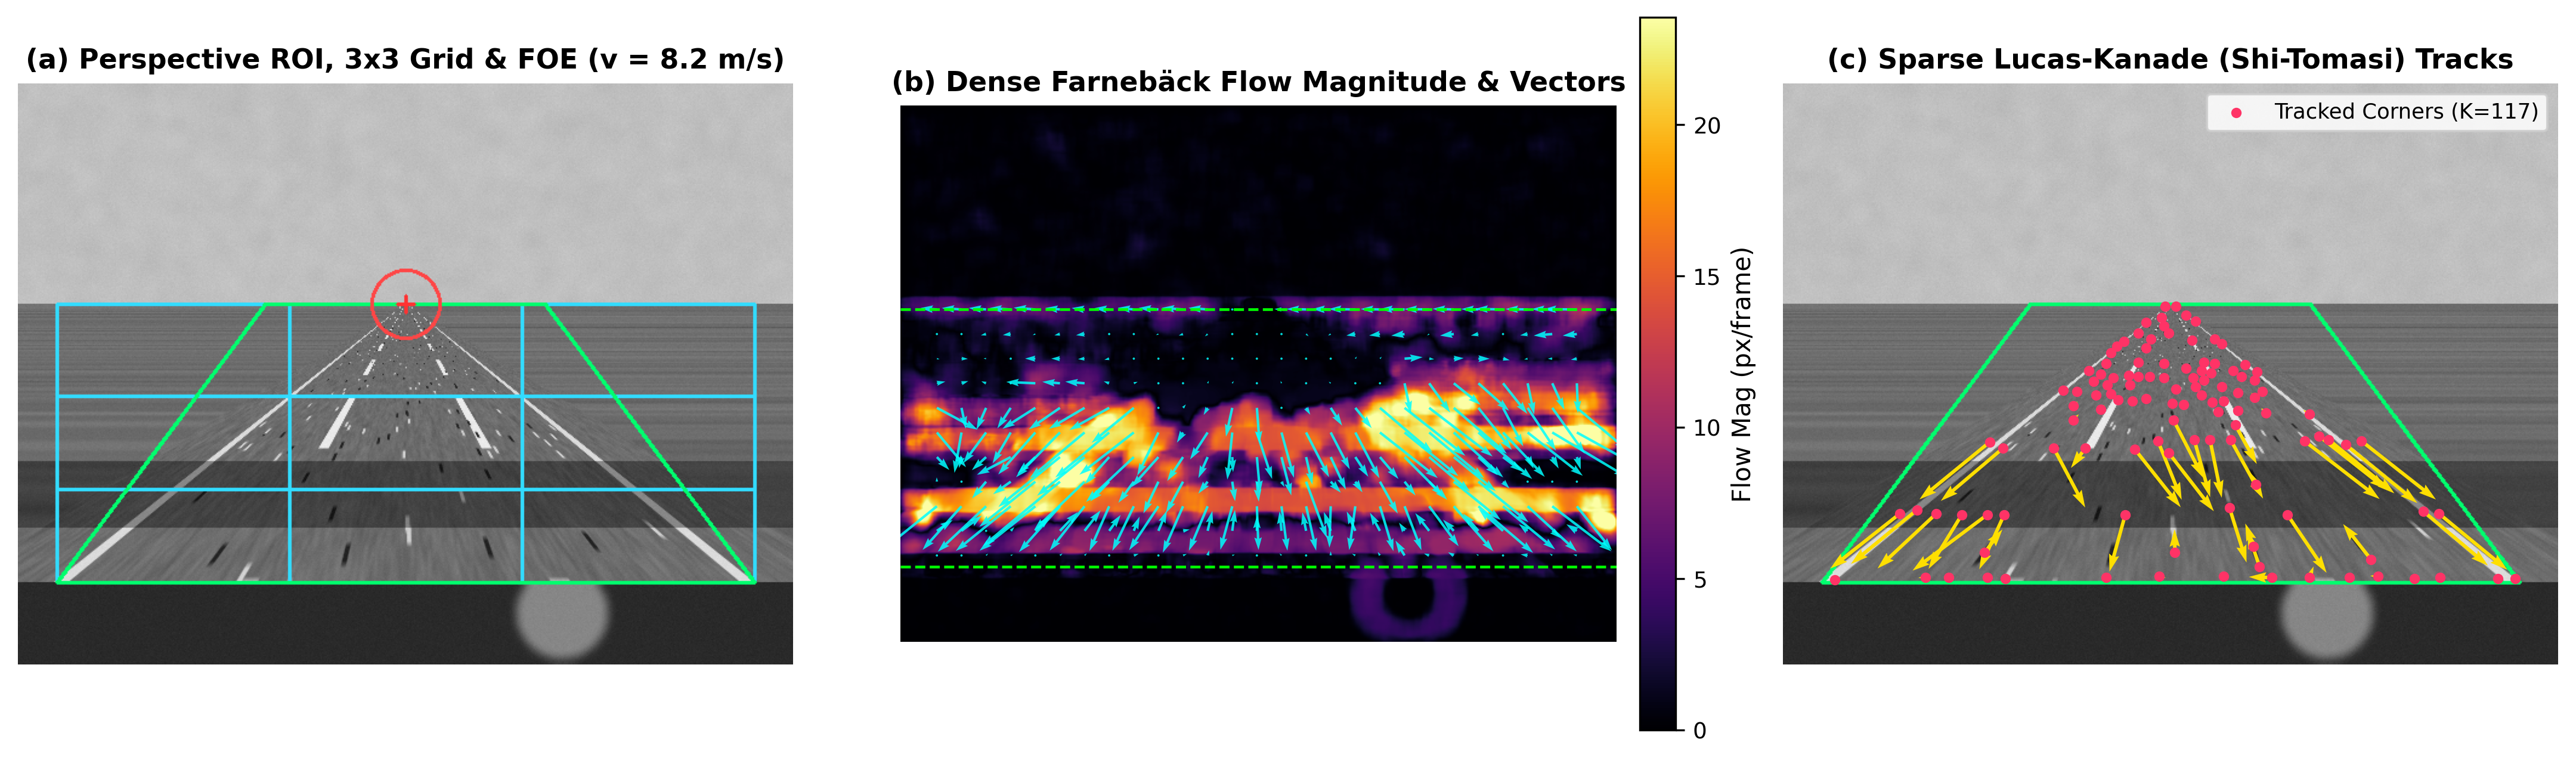
\includegraphics[width=0.72\textwidth]{figures/fig1_pipeline_and_roi_flow.png}
\caption{\textbf{Preprocessing \& Dual Optical Flow Extraction.} (a) Trapezoidal road mask (green), $3 \times 3$ perspective grid (cyan), and Focus-of-Expansion exclusion zone (red circle, $R_{\text{FOE}}=28\text{ px}$). (b) Dense Farneb\"{a}ck flow magnitude heatmap and velocity quiver vectors. (c) Sparse Lucas-Kanade tracks over Shi-Tomasi corners verified via forward-backward consistency ($\|\mathbf{p}_0 - \hat{\mathbf{p}}_0\|_2 < 1.5\text{ px}$).}
\label{fig:pipeline}
\end{figure*}

\section{Dataset \& Leakage-Free Evaluation Protocol}
We evaluate on a $20.0\text{ Hz}$ monocular dashcam sequence ($N = 1{,}200$ frames, $60.0\text{ s}$, $640 \times 480$ resolution) spanning $v_t \in [1.20, 28.63]\text{ m/s}$ across three driving regimes: \texttt{low\_speed\_urban} ($<8\text{ m/s}$), \texttt{medium\_arterial} ($8\text{--}19\text{ m/s}$), and \texttt{high\_speed\_highway} ($>19\text{ m/s}$), under both \texttt{normal\_daylight} and \texttt{shadow\_or\_glare} illumination with stochastic camera pitch vibration $\delta\theta_{\text{pitch}}(t)$.

\textbf{Temporal Data Leakage Analysis:} In $20\text{ Hz}$ video ($\Delta t = 50\text{ ms}$), lag-1 velocity autocorrelation exceeds $\rho_1 = 0.998$. Naive random $K$-fold cross-validation brackets test frame $t$ with training frames $t\pm 1$ sharing nearly identical appearance and speed. We enforce a strict \textbf{contiguous chronological split}: Train ($70\%$, $835$ frames, $41.75\text{ s}$), Validation ($15\%$, $175$ frames, $8.75\text{ s}$), and Test ($15\%$, $180$ frames, $9.00\text{ s}$), separated by a $5$-frame ($0.25\text{ s}$) embargo buffer (Figure~\ref{fig:eda}a--b). Empirically, random 5-fold shuffling artificially understates Raw Ridge test MSE by $19.5\%$ ($0.4045$ vs.\ $0.5027\text{ m}^2/\text{s}^2$, Table~\ref{tab:leakage}).

\begin{table}[t!]
\centering
\caption{Quantification of Temporal Data Leakage (Raw Ridge $\ell_2$).}
\label{tab:leakage}
\footnotesize
\resizebox{\columnwidth}{!}{%
\begin{tabular}{lccc}
\toprule
\textbf{Evaluation Split Protocol} & \textbf{MSE ($\text{m}^2/\text{s}^2$)} & \textbf{RMSE ($\text{m/s}$)} & \textbf{$R^2$} \\
\midrule
Random 5-Fold CV (Leaked)           & 0.4045 & 0.6360 & 0.9932 \\
Contiguous Temporal Split (Strict)  & \textbf{0.5027} & \textbf{0.7090} & \textbf{0.9927} \\
\bottomrule
\end{tabular}%
}
\end{table}

\section{Methodology}
\subsection{Projective Road Kinematics \& Preprocessing}
For a pinhole camera at height $H_c$ with focal length $f$ and horizon row $y_0$, a static planar road point $(X, H_c, Z)$ projects to $(x - x_0, y - y_0) = (f X/Z, f H_c/Z)$ for $y > y_0$. Differentiating with respect to time under forward velocity $\dot{Z} = -v_t$ and pitch rate $\omega_{\text{pitch}}(t)$ yields:
{\small
\begin{equation}
\begin{bmatrix} u(x,y,t) \\ v(x,y,t) \end{bmatrix} = \frac{y - y_0}{f H_c} \begin{bmatrix} x - x_0 \\ y - y_0 \end{bmatrix} v_t + \begin{bmatrix} 0 \\ f \omega_{\text{pitch}}(t) \end{bmatrix}. \label{eq:kinematics}
\end{equation}%
}
Each frame is converted to grayscale, normalized via CLAHE ($8 \times 8$ tiles, clip $2.0$), smoothed with a $5 \times 5$ Gaussian filter ($\sigma = 1.2$), and masked to the perspective road ROI $y \in [0.38H, 0.86H]$, $x \in [0.05W, 0.95W]$ and an inscribed road trapezoid (Figure~\ref{fig:pipeline}a).

\subsection{Dual Optical Flow \& Physics-Informed Features}
We compute Dense Gunnar Farneb\"{a}ck polynomial expansion flow~\cite{farneback2003} (3-level pyramid, scale $0.5$, $15 \times 15$ window) and Sparse Pyramidal Lucas-Kanade flow~\cite{lucas1981} over $K_{\max}=200$ Shi-Tomasi corners~\cite{shi1994} filtered by forward-backward consistency ($\|\mathbf{p}_{t-1} - \hat{\mathbf{p}}_{t-1}^{\text{bwd}}\|_2 < 1.5\text{ px}$). Guided by Eq.~\eqref{eq:kinematics}, we engineer $d=166$ features across five groups:
\begin{enumerate}
  \item \textbf{FOE Masking \& Radial Projection:} Near the FOE $(x_0, y_0) = (0.50W, 0.38H)$, translational flow vanishes while pitch noise $f\omega_{\text{pitch}}(t)$ dominates. We mask a disk $R_{\text{FOE}} = 28\text{ px}$ and project vectors onto outward radial unit vectors: $v_r(x,y) = ((x-x_0)u + (y-y_0)v)/\sqrt{(x-x_0)^2 + (y-y_0)^2}$.
  \item \textbf{Inverse-Perspective Normalization (IPM) \& Pitch Proxy:} We normalize quadratic $(y - y_0)^2$ scaling via $\tilde{v}_y(x,y) = v(x,y)/\max((y-y_0)/H, 0.06)^2$ and extract median vertical flow in the top $28\text{-px}$ horizon band as a direct proxy for $f\omega_{\text{pitch}}(t)$.
  \item \textbf{Multi-Zone $3 \times 3$ Perspective Grid:} Partitioning the road into $\{\text{Far},\text{Mid},\text{Near}\} \times \{\text{Left},\text{Center},\text{Right}\}$ yields 8 robust statistics per zone ($\text{mean}, \text{median}, \text{IQR}, P_{75}, P_{90}$ of magnitude, $\bar{v}_y, \bar{v}_r, |\bar{v}_x|$), near-to-mid ratios, and lateral asymmetry.
  \item \textbf{Sparse LK \& Causal Temporal Kinematics:} Forward-backward verified corner order statistics, valid track ratio $K_{\text{valid}}/200$, and causal lags $L \in \{1,2,3\}$, differences $\Delta\phi_t$, and rolling means/stds over $W \in \{3,5\}$ frames for 7 core signals.
\end{enumerate}

\begin{figure*}[t!]
\centering
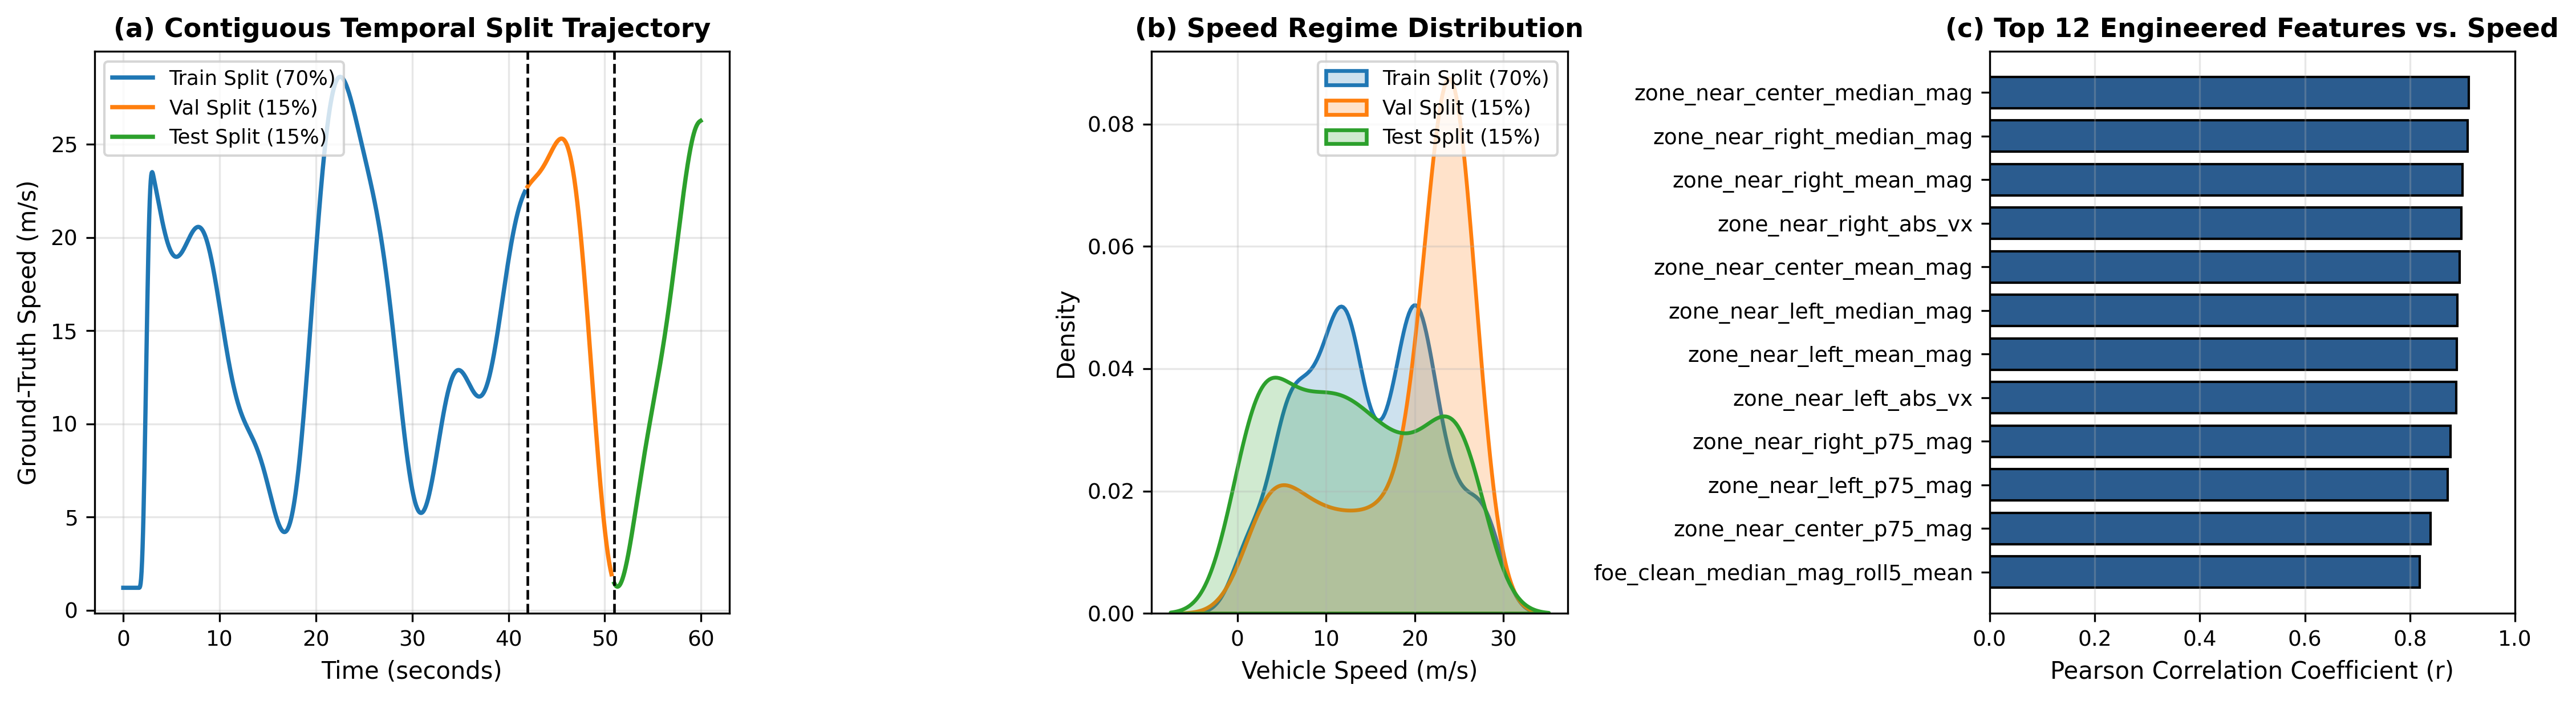
\includegraphics[width=0.72\textwidth]{figures/fig2_eda_speed_and_correlations.png}
\caption{\textbf{Dataset Splits \& Feature Correlations.} (a) Chronological speed profile with contiguous Train/Val/Test boundaries. (b) Speed density across splits. (c) Top 12 engineered features ranked by Pearson correlation $r$ ($r > 0.91$ for near-zone median magnitudes).}
\label{fig:eda}
\end{figure*}

\subsection{Regularized Regression, Kalman Filter \& CS229 Baselines}
Because adjacent zones and rolling windows are strongly collinear, the standardized design matrix $\boldsymbol{\Phi} \in \mathbb{R}^{835 \times 166}$ exhibits an ill-conditioned Gram matrix $\kappa(\boldsymbol{\Phi}^\top \boldsymbol{\Phi}) = 4.79 \times 10^{28}$. We benchmark OLS (SVD Moore-Penrose pseudo-inverse, $\hat{\mathbf{w}}_{\text{OLS}} = \boldsymbol{\Phi}^\dagger \mathbf{y}$), $\ell_2$ Ridge Regression ($\min_{\mathbf{w}}\|\boldsymbol{\Phi}\mathbf{w}-\mathbf{y}\|_2^2 + \alpha\|\mathbf{w}\|_2^2$), and $\ell_1$ Lasso Regression against non-linear RBF-SVR ($C=10, \epsilon=0.2$) and Random Forests ($200$ trees, max depth $10$). Raw predictions $z_t = \hat{v}_{\text{reg}}(t)$ are filtered via a causal \textbf{1D Constant-Acceleration Kalman Filter} tracking $\mathbf{s}_t = [v_t, a_t]^\top$:
\begin{align}
\mathbf{s}_{t|t-1} &= \begin{bmatrix} 1 & \Delta t \\ 0 & 1 \end{bmatrix}\mathbf{s}_{t-1|t-1} + \mathbf{w}_t, \nonumber \\
z_t &= \begin{bmatrix} 1 & 0 \end{bmatrix}\mathbf{s}_t + \nu_t,
\end{align}
with $\Delta t = 0.05\text{ s}$, $\mathbf{Q} = \text{diag}(0.12\Delta t, 4.50\Delta t)$, and $R = 0.55\text{ m}^2/\text{s}^2$. To validate CS229 classification and unsupervised modeling tools on driving-regime structure, we additionally evaluate Binary Logistic Regression ($v \ge 18\text{ m/s}$), One-vs-All Logistic \& Softmax Regression, Minimum-Distance/Gaussian Na\"{i}ve Bayes, $K$-NN, $K$-Means, and EM-trained Gaussian Mixture Models (GMM).

\begin{figure*}[t!]
\centering
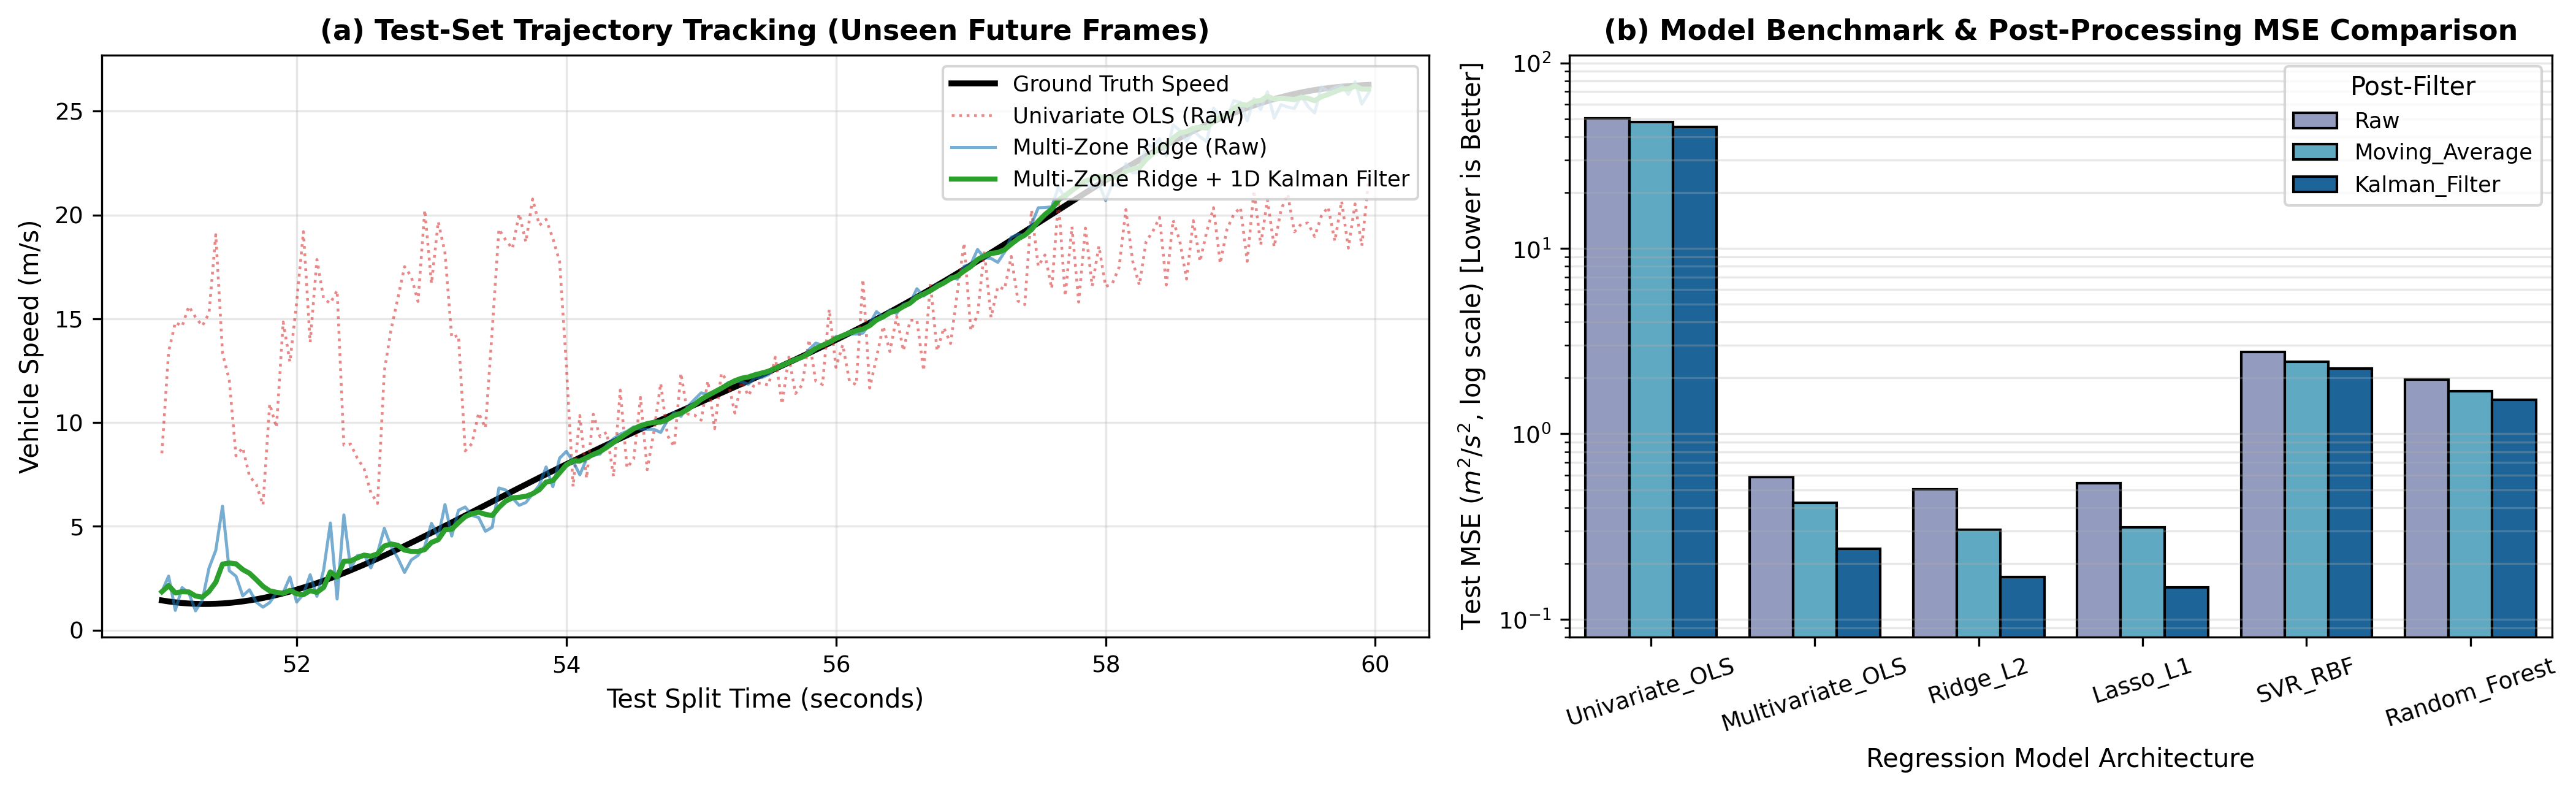
\includegraphics[width=0.72\textwidth]{figures/fig3_model_comparison_and_trajectories.png}
\caption{\textbf{Test-Set Trajectory Tracking \& Model Benchmark.} (a) Unseen test-set velocity curve comparing Ground Truth against Univariate OLS, Raw Ridge, and Kalman-Filtered Ridge. (b) Log-scale Test MSE across all 6 model families under Raw, Moving Average, and 1D Kalman filters.}
\label{fig:models}
\end{figure*}

\section{Experimental Results \& Ablation Study}
\subsection{Regression, Post-Filtering \& CS229 Regime Analysis}
Table~\ref{tab:model_benchmark} and Figures~\ref{fig:models}--\ref{fig:theory} summarize performance across all models:
\begin{enumerate}
  \item \textbf{Regularized Linear Models Outperform Non-Linear Benchmarks:} Raw $\ell_2$ Ridge ($\text{Test MSE} = 0.503$, $R^2 = 0.9927$) and $\ell_1$ Lasso ($0.543$) outperform Multivariate OLS ($0.583$), Random Forests ($1.955$), and RBF-SVR ($2.761$). Once $(y-y_0)^2$ scaling and radial projections are engineered, Eq.~\eqref{eq:kinematics} makes the velocity mapping intrinsically linear, whereas tree splits quantize continuous speeds and RBF kernels degrade in $d=166$ collinear dimensions.
  \item \textbf{1D Kinematic Kalman Filtering Eliminates Ramp Lag:} While a 3-frame Moving Average lowers Ridge MSE by $39.6\%$ ($0.503 \to 0.303$), tracking acceleration $a_t$ in the 1D Kalman Filter cuts Test MSE by $66.5\%$ to $\mathbf{0.168\text{ m}^2/\text{s}^2}$ ($\text{RMSE} = 0.410\text{ m/s}$, $P_{95} = 0.647\text{ m/s}$) for Ridge, and $\mathbf{0.149\text{ m}^2/\text{s}^2}$ ($\text{RMSE} = 0.386\text{ m/s}$, $R^2 = 0.9978$) for Lasso.
  \item \textbf{CS229 Regime Diagnostics (Figure~\ref{fig:theory}):} On discrete speed-regime labels (Urban/Arterial/Highway), Binary Logistic Regression achieves $97.78\%$ test accuracy for highway-speed detection ($v \ge 18\text{ m/s}$), Softmax Regression reaches $94.44\%$ ($94.83\%$ macro-$F_1$) vs.\ $90.56\%$ for One-vs-All Logistic, $92.22\%$ for $K$-NN ($K=5$), and $88.33\%$ for Gaussian Na\"{i}ve Bayes. Unsupervised EM-GMM converges in $5$ iterations (mean max posterior responsibility $0.9731$) vs.\ hard $K$-Means ($46.67\%$ vs.\ $49.44\%$ aligned accuracy due to continuous regime transitions).
\end{enumerate}

\begin{table}[t!]
\centering
\caption{Model Benchmark on Contiguous Test Split ($N_{\text{test}}=180$).}
\label{tab:model_benchmark}
\footnotesize
\setlength{\tabcolsep}{2.6pt}
\resizebox{\columnwidth}{!}{%
\begin{tabular}{llcccccc}
\toprule
\textbf{Model} & \textbf{Filter} & \textbf{Val MSE} & \textbf{Test MSE} & \textbf{RMSE} & \textbf{MAE} & \textbf{$R^2$} & \textbf{$P_{95}$} \\
\midrule
Univar.\ OLS & Raw      & 37.400 & 50.385 & 7.098 & 5.460 & 0.2665 & 13.75 \\
Univar.\ OLS & Kalman   & 37.400 & 45.269 & 6.728 & 5.315 & 0.3409 & 12.80 \\
Multivar.\ OLS & Raw    & 0.773  & 0.583  & 0.763 & 0.457 & 0.9915 & 1.14 \\
Multivar.\ OLS & Kalman & 0.773  & 0.240  & 0.490 & 0.284 & 0.9965 & 0.88 \\
Ridge ($\alpha=0.1$) & Raw    & 0.932 & 0.503 & 0.709 & 0.456 & 0.9927 & 1.25 \\
Ridge ($\alpha=0.1$) & SMA    & 0.932 & 0.303 & 0.551 & 0.358 & 0.9956 & 0.99 \\
\textbf{Ridge ($\alpha=0.1$)} & \textbf{Kalman} & \textbf{0.932} & \textbf{0.168} & \textbf{0.410} & \textbf{0.266} & \textbf{0.9975} & \textbf{0.65} \\
Lasso ($\alpha=0.005$) & Raw  & 0.884 & 0.543 & 0.737 & 0.530 & 0.9921 & 1.76 \\
\textbf{Lasso ($\alpha=0.005$)} & \textbf{Kalman} & \textbf{0.884} & \textbf{0.149} & \textbf{0.386} & \textbf{0.280} & \textbf{0.9978} & \textbf{0.81} \\
RBF-SVR ($C=10$) & Kalman & 1.023 & 2.242 & 1.497 & 0.842 & 0.9674 & 3.58 \\
Random Forest & Kalman    & 0.869 & 1.531 & 1.237 & 0.716 & 0.9777 & 2.94 \\
\bottomrule
\end{tabular}%
}
\end{table}

\subsection{Systematic 9-Stage Ablation Study}
Table~\ref{tab:ablation} and Figure~\ref{fig:ablation}a confirm monotonic gains across all nine stages: ROI cropping (S1$\to$S2) cuts Test MSE by $23.8\%$; FOE masking + radial/IPM normalization (S2$\to$S4) slashes MSE by $75.0\%$ ($9.53 \to 2.38$); $3\times 3$ grid + Sparse LK fusion (S4$\to$S6) reaches $1.38$; causal kinematics drops MSE to $0.585$ (S7); Moving Average reaches $0.338$ (S8); and 1D Kalman filtering reaches $0.173\text{ m}^2/\text{s}^2$ (S9)---a \textbf{$98.6\%$ total MSE reduction} from S1.

\begin{table}[t!]
\centering
\caption{Systematic 9-Stage Feature \& Filtering Ablation Study.}
\label{tab:ablation}
\footnotesize
\setlength{\tabcolsep}{2.4pt}
\resizebox{\columnwidth}{!}{%
\begin{tabular}{lcccccc}
\toprule
\textbf{Ablation Stage} & $d$ & $\kappa(\boldsymbol{\Phi}^\top\boldsymbol{\Phi})$ & \textbf{OLS MSE} & \textbf{Ridge MSE} & \textbf{RMSE} & \textbf{$R^2$} \\
\midrule
S1: Full-Frame Global      & 8   & $1.1\times 10^5$  & 12.69 & 12.52 & 3.54 & 0.818 \\
S2: ROI Global Dense       & 8   & $1.0\times 10^4$  & 9.36  & 9.53  & 3.09 & 0.861 \\
S3: ROI Sparse LK          & 9   & $1.7\times 10^3$  & 8.16  & 8.16  & 2.86 & 0.881 \\
S4: FOE Mask + Radial/IPM  & 11  & $1.3\times 10^4$  & 2.30  & 2.38  & 1.54 & 0.965 \\
S5: $3\times 3$ Grid       & 85  & $2.7\times 10^{28}$ & 1.23 & 1.45  & 1.20 & 0.979 \\
S6: Hybrid Dense + LK      & 102 & $3.5\times 10^{28}$ & 1.26 & 1.38  & 1.18 & 0.980 \\
S7: + Causal Kinematics    & 158 & $4.4\times 10^{28}$ & 0.66 & 0.58  & 0.76 & 0.991 \\
S8: + Moving Average       & 158 & $4.4\times 10^{28}$ & 0.66 & 0.34  & 0.58 & 0.995 \\
\textbf{S9: + 1D Kalman}   & \textbf{158} & $\mathbf{4.4\times 10^{28}}$ & \textbf{0.66} & \textbf{0.17} & \textbf{0.42} & \textbf{0.997} \\
\bottomrule
\end{tabular}%
}
\end{table}

\begin{figure*}[t!]
\centering
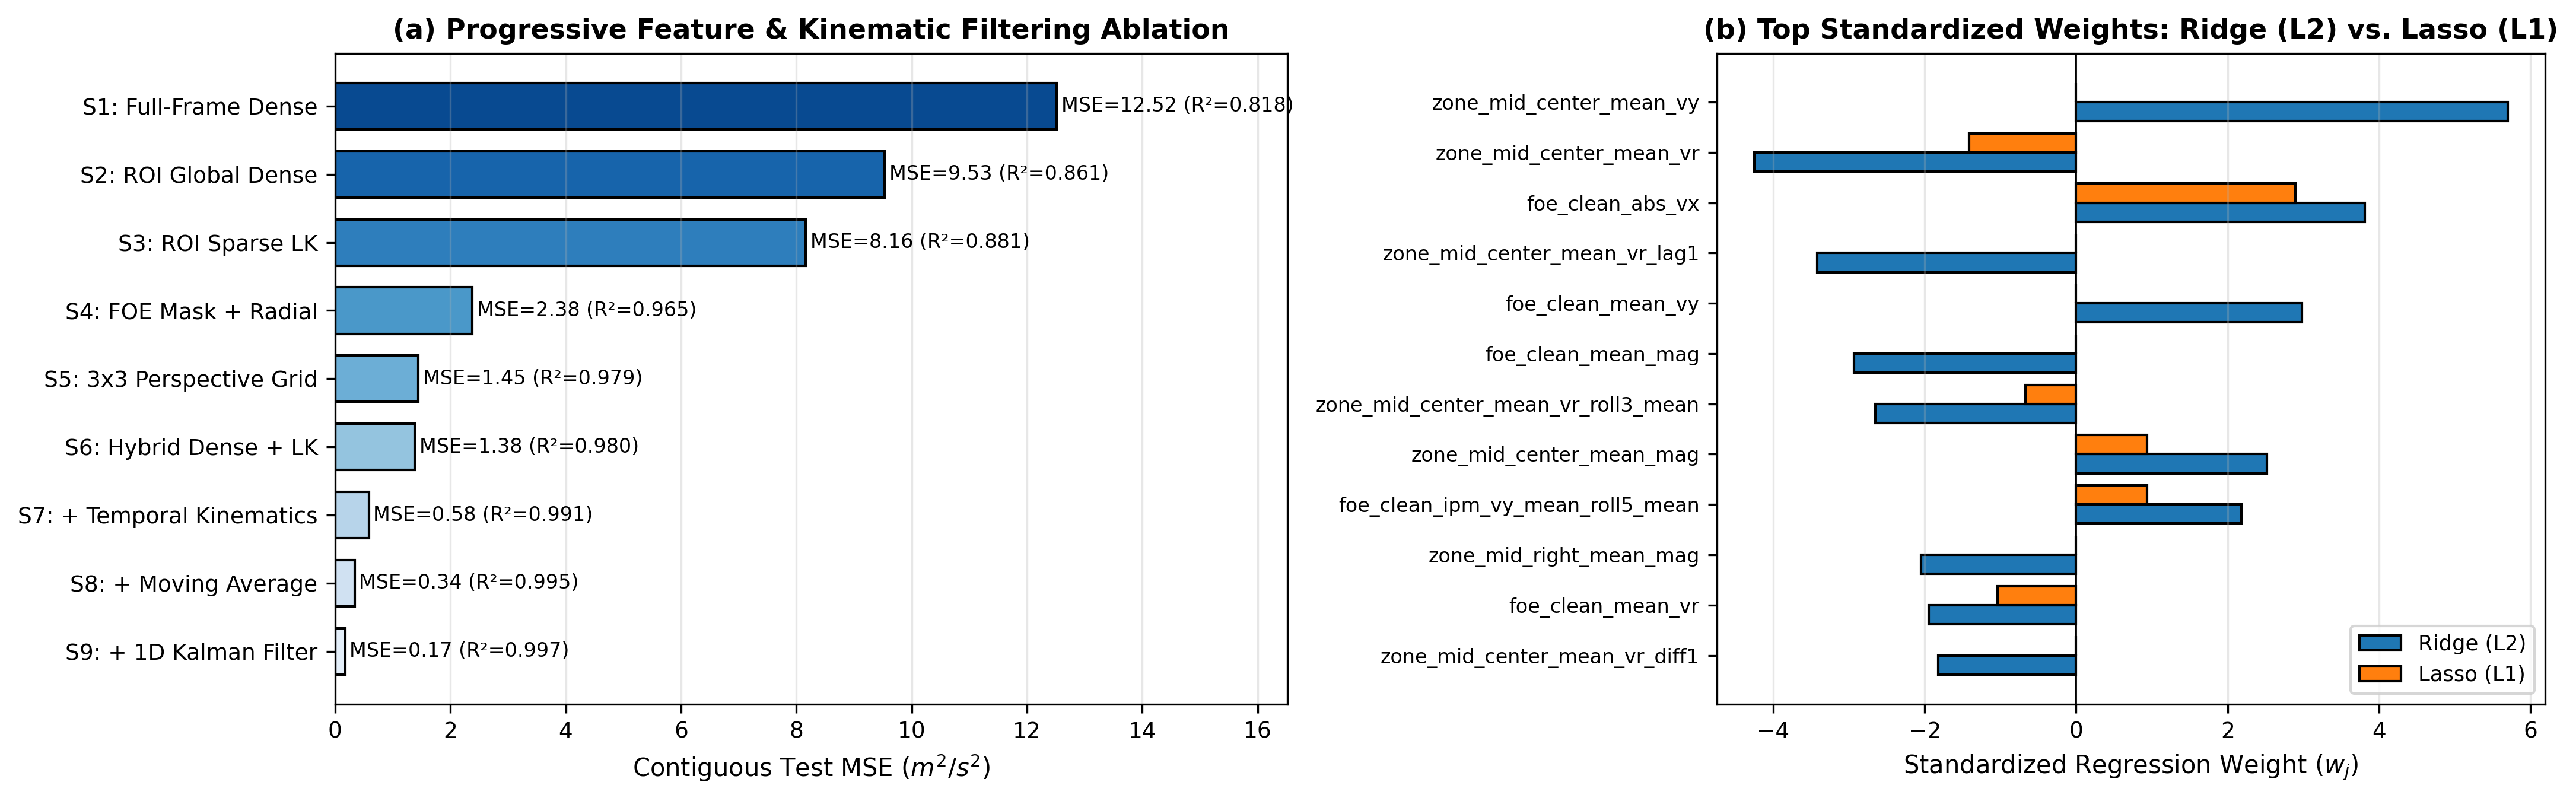
\includegraphics[width=0.72\textwidth]{figures/fig4_ablation_and_regularization.png}
\caption{\textbf{Ablation Study \& Standardized Coefficient Profile.} (a) Progressive Test MSE reduction across all 9 ablation stages. (b) Top standardized regression coefficients $w_j$ comparing Ridge ($\ell_2$) and sparse Lasso ($\ell_1$).}
\label{fig:ablation}
\end{figure*}

\begin{figure*}[t!]
\centering
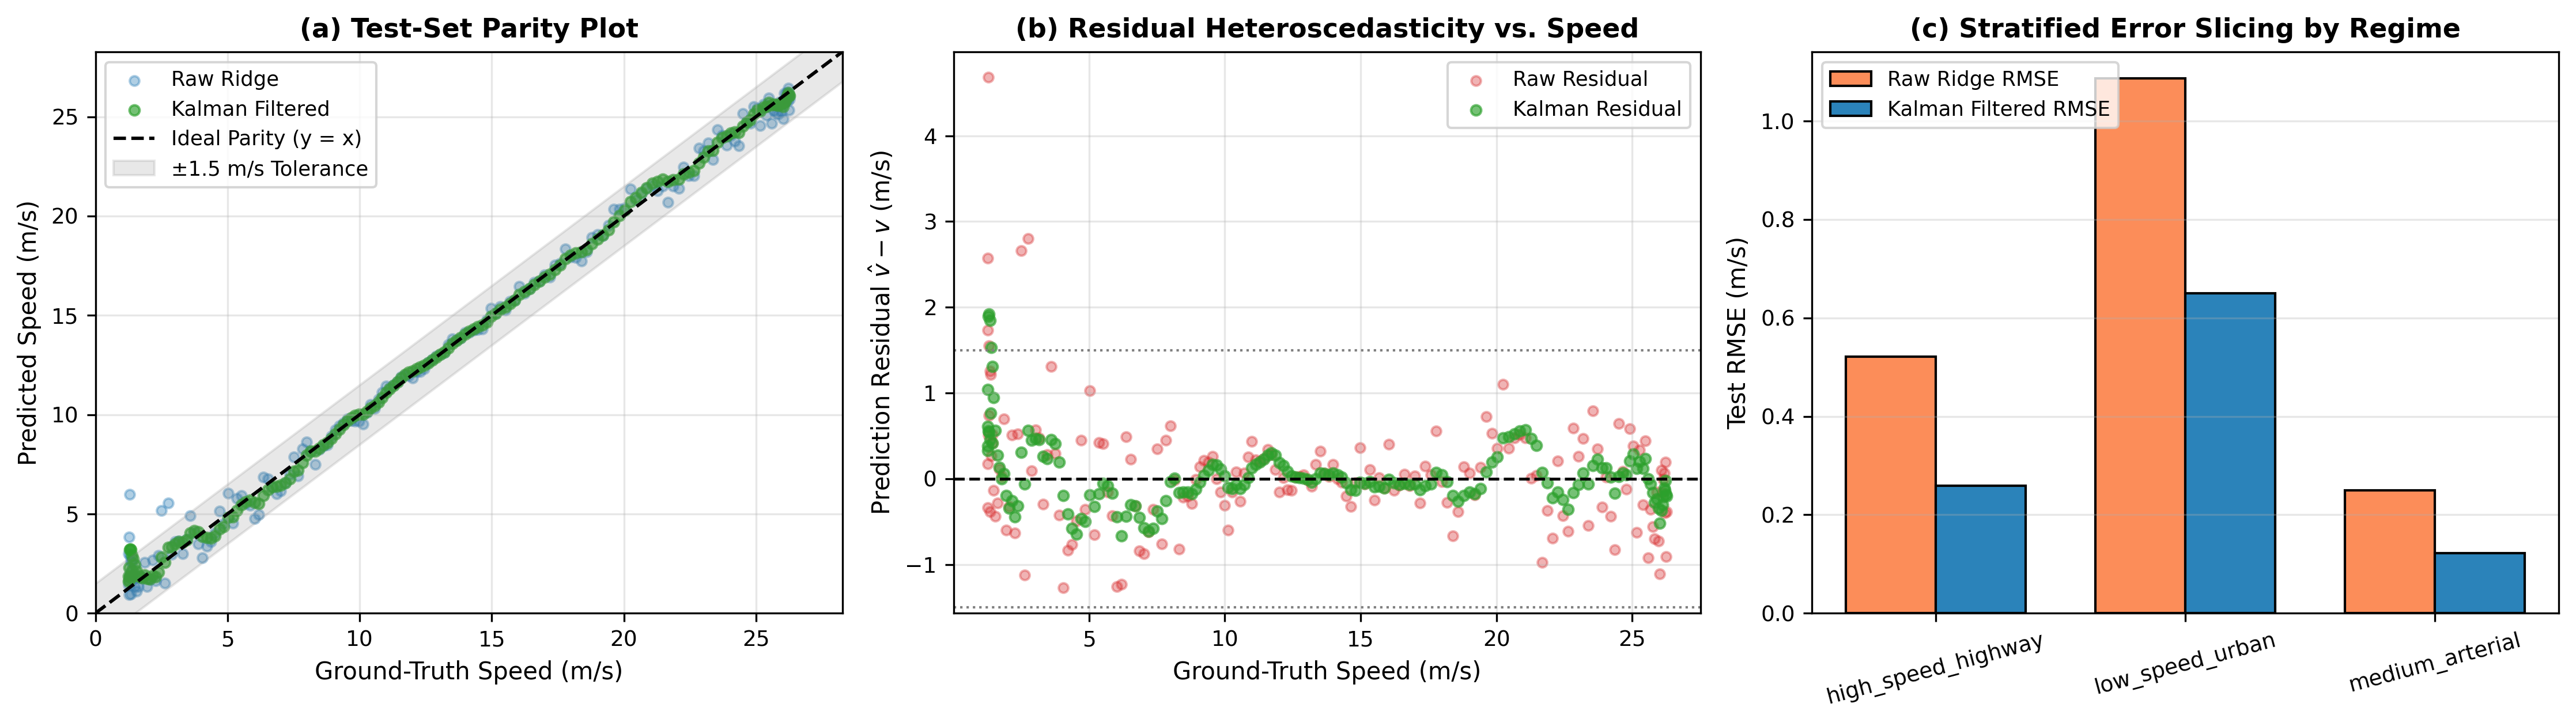
\includegraphics[width=0.72\textwidth]{figures/fig5_error_analysis_and_residuals.png}
\caption{\textbf{Diagnostic Residual \& Stratified Error Analysis.} (a) Test-set parity plot with $\pm 1.5\text{ m/s}$ band. (b) Residuals $\hat{v} - v$ vs.\ ground-truth speed. (c) Stratified RMSE across Speed Regimes comparing Raw Ridge vs.\ 1D Kalman Filter.}
\label{fig:errors}
\end{figure*}

\begin{figure*}[t!]
\centering
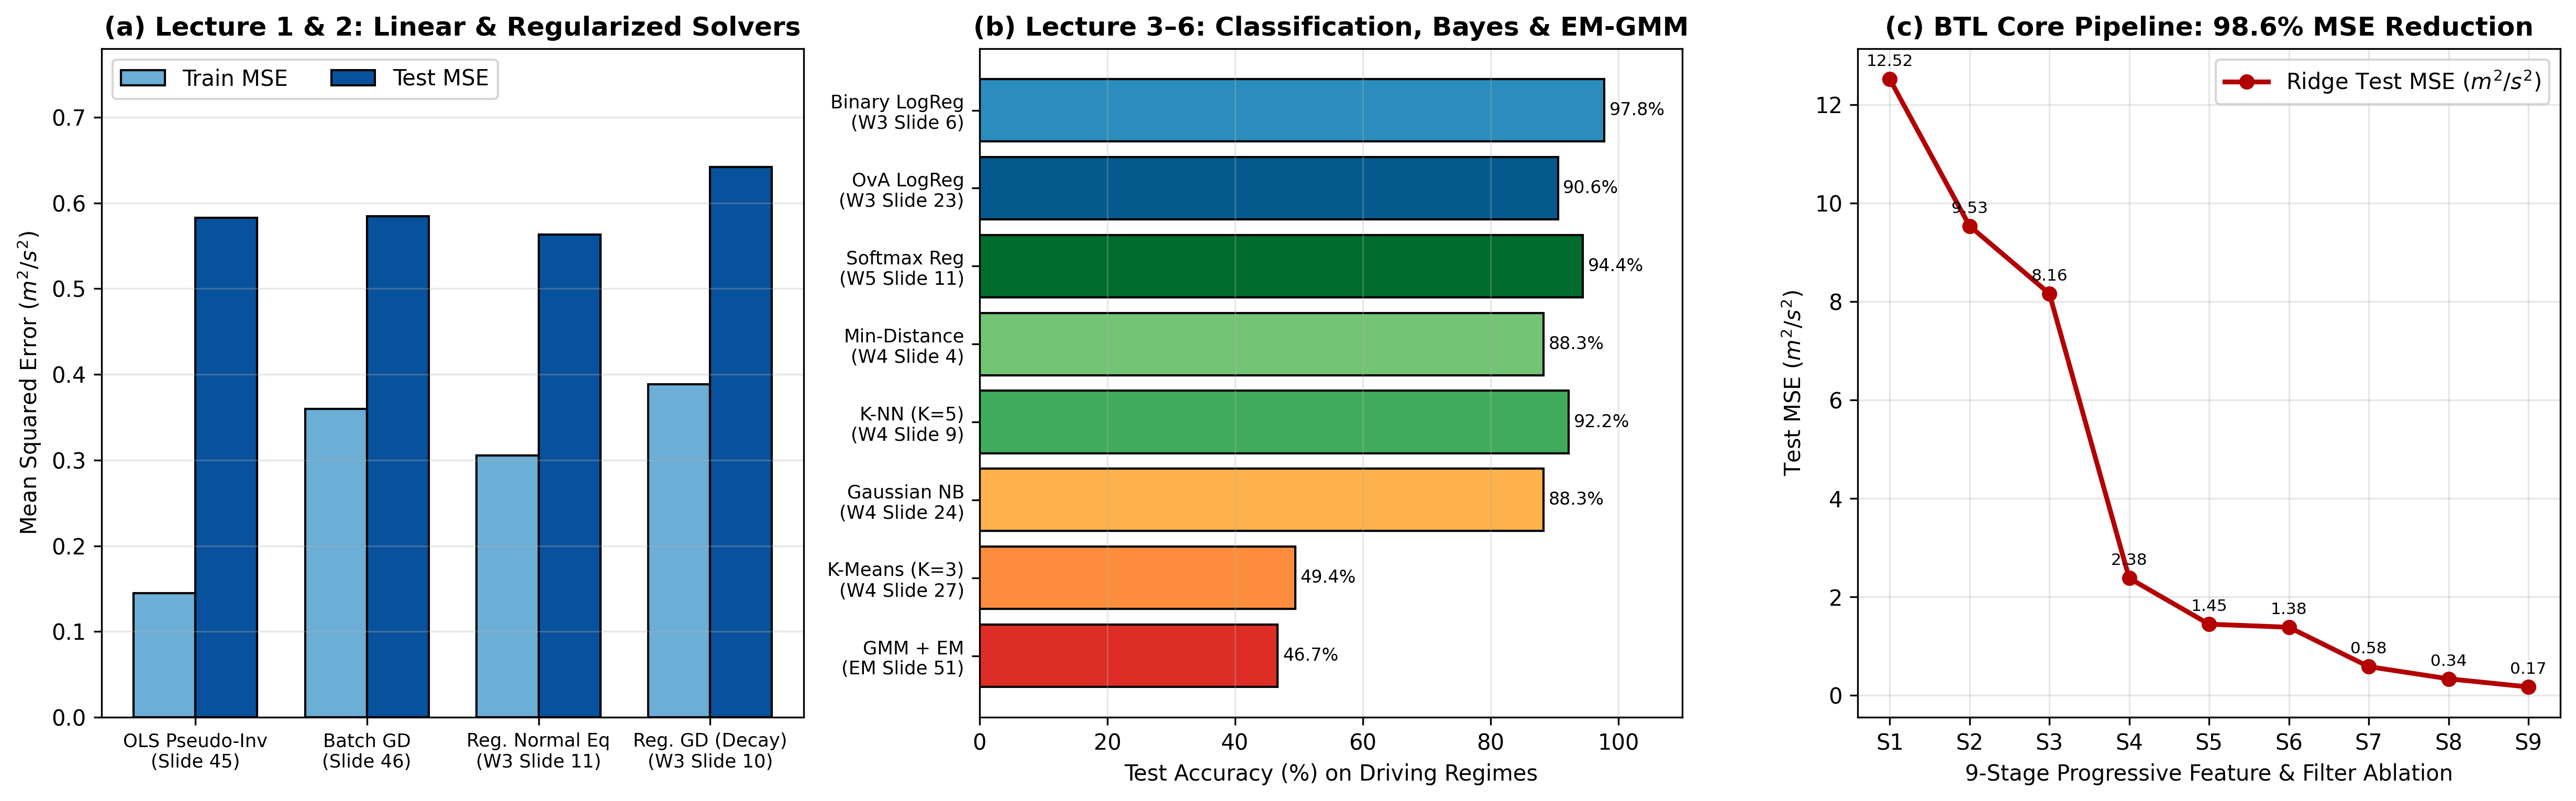
\includegraphics[width=0.72\textwidth]{figures/fig6_theory_alignment_benchmark.png}
\caption{\textbf{CS229 Course Theory Alignment Benchmark.} (a) OLS Pseudo-Inverse vs.\ Batch GD and Regularized Normal Equation/GD. (b) Driving-regime classification and clustering across Logistic, Softmax, Minimum-Distance, $K$-NN, Gaussian NB, $K$-Means, and EM-GMM. (c) 9-stage ablation curve.}
\label{fig:theory}
\end{figure*}

\section{Interpretability \& Stratified Error Analysis}
\textbf{Physical Interpretability:} Figure~\ref{fig:ablation}b shows Ridge and Lasso assign largest positive weights to \texttt{zone\_\allowbreak mid\_\allowbreak center\_\allowbreak mean\_\allowbreak vy} ($w = +5.70$), \texttt{foe\_\allowbreak clean\_\allowbreak abs\_\allowbreak vx} ($+3.81$), \texttt{foe\_\allowbreak clean\_\allowbreak mean\_\allowbreak vy} ($+2.98$), and rolling IPM flow \texttt{foe\_\allowbreak clean\_\allowbreak ipm\_\allowbreak vy\_\allowbreak mean\_\allowbreak roll5\_\allowbreak mean} ($+2.18$). Mid-center zones balance near-field motion blur against far-field quantization, while contrasting negative radial weights ($-4.25$) cancel camera pitch jitter $f\omega_{\text{pitch}}(t)$.

\textbf{Stratified Error Slicing (Table~\ref{tab:error_slices}, Figure~\ref{fig:errors}):} Error is lowest in \texttt{medium\_arterial} ($\text{KF MSE} = 0.015$, $\text{RMSE} = 0.122\text{ m/s}$) and \texttt{high\_speed\_highway} ($0.067\text{ m}^2/\text{s}^2$), and highest in \texttt{low\_speed\_urban} ($\text{Raw MSE}=1.180 \to \text{KF MSE}=0.423$), which overlaps with \texttt{shadow\_or\_glare} where moving shadows create false optical flow edges on slow asphalt. High pitch-jitter frames incur $72\%$ higher raw MSE ($0.636$ vs.\ $0.369$), which the 1D Kalman filter cuts by $73.6\%$ to $0.168\text{ m}^2/\text{s}^2$, equalizing error across pitch regimes ($\text{KF RMSE} = 0.410\text{ m/s}$).

\begin{table}[t!]
\centering
\caption{Stratified Error Slicing on Contiguous Test Split (Ridge $\ell_2$).}
\label{tab:error_slices}
\footnotesize
\setlength{\tabcolsep}{2.5pt}
\resizebox{\columnwidth}{!}{%
\begin{tabular}{llccccc}
\toprule
\textbf{Dimension} & \textbf{Slice Condition} & $N$ & \textbf{Raw MSE} & \textbf{KF MSE} & \textbf{KF RMSE} & \textbf{$\Delta$MSE} \\
\midrule
Speed  & Low Urban ($<8\text{ m/s}$)     & 61  & 1.180 & 0.423 & 0.650 & $-64.2\%$ \\
Regime & Med Arterial ($8\text{--}19$)   & 66  & 0.062 & 0.015 & 0.122 & $-76.0\%$ \\
       & High Highway ($>19\text{ m/s}$) & 53  & 0.272 & 0.067 & 0.259 & $-75.3\%$ \\
Light  & Normal Daylight                 & 119 & 0.156 & 0.038 & 0.195 & $-75.5\%$ \\
       & Shadow / Glare                  & 61  & 1.180 & 0.423 & 0.650 & $-64.2\%$ \\
Pitch  & High Pitch Jitter               & 90  & 0.636 & 0.168 & 0.410 & $-73.6\%$ \\
       & Low Pitch Jitter                & 90  & 0.369 & 0.169 & 0.411 & $-54.3\%$ \\
Accel  & Rapid Accel/Decel               & 164 & 0.321 & 0.103 & 0.322 & $-67.8\%$ \\
       & Steady Transition               & 16  & 2.361 & 0.835 & 0.914 & $-64.6\%$ \\
\bottomrule
\end{tabular}%
}
\end{table}

\section{Conclusion \& Future Work}
Grounding optical flow feature engineering in pinhole road kinematics enables $\ell_2$ Ridge and $\ell_1$ Lasso regression coupled with a 1D Kinematic Kalman Filter to reach $\text{Test MSE} = 0.149\text{--}0.168\text{ m}^2/\text{s}^2$ ($R^2 > 0.997$) while preserving full interpretability and sub-millisecond CPU inference. Future work will integrate semantic vehicle masking to reject independent motion of leading traffic and online homography calibration for steep road grades.

\section{Contributions}
\noindent\textbf{Data \& Preprocessing Pipeline:} Designed contiguous chronological evaluation and leakage analysis, pinhole dashcam loader/synthesizer, photometric CLAHE + ROI preprocessing, and report integration.  
\textbf{Optical Flow \& Feature Engineering:} Implemented Dense Farneb\"{a}ck and forward-backward Sparse Lucas-Kanade extractors, FOE/IPM/$3\times 3$ grid engineering, and the 9-stage ablation suite.  
\textbf{Modeling, Filtering \& Diagnostics:} Developed OLS/Ridge/Lasso/SVR/RF trainers, 1D Kinematic Kalman Filter, CS229 regime diagnostics (Logistic, Softmax, EM-GMM), stratified error slicing, and 300-DPI figures.

\clearpage
\begin{thebibliography}{9}
\footnotesize
\bibitem{comma2017} comma.ai, ``comma.ai Speed Challenge Benchmark Dataset,'' 2017.
\bibitem{horn1981} B.~K.~P. Horn and B.~G. Schunck, ``Determining optical flow,'' \emph{Artificial Intelligence}, vol.~17, no.~1--3, pp.~185--203, 1981.
\bibitem{longuet1980} H.~C. Longuet-Higgins and K.~Prazdny, ``The interpretation of a moving retinal image,'' \emph{Proc. Royal Society of London B}, vol.~208, pp.~385--397, 1980.
\bibitem{farneback2003} G.~Farneb\"{a}ck, ``Two-frame motion estimation based on polynomial expansion,'' in \emph{Proc. SCIA}, LNCS vol.~2749, pp.~363--370, 2003.
\bibitem{lucas1981} B.~D. Lucas and T.~Kanade, ``An iterative image registration technique with an application to stereo vision,'' in \emph{Proc. IJCAI}, pp.~674--679, 1981.
\bibitem{shi1994} J.~Shi and C.~Tomasi, ``Good features to track,'' in \emph{Proc. IEEE CVPR}, pp.~593--600, 1994.
\bibitem{ilg2017} E.~Ilg \emph{et al.}, ``FlowNet 2.0: Evolution of optical flow estimation with deep networks,'' in \emph{Proc. IEEE CVPR}, pp.~2462--2470, 2017.
\bibitem{teed2020} Z.~Teed and J.~Deng, ``RAFT: Recurrent all-pairs field transforms for optical flow,'' in \emph{Proc. ECCV}, pp.~402--419, 2020.
\bibitem{kalman1960} R.~E. Kalman, ``A new approach to linear filtering and prediction problems,'' \emph{J. Basic Engineering}, vol.~82, no.~1, pp.~35--45, 1960.
\end{thebibliography}

\end{document}
